\documentclass[9pt]{extarticle}%
\usepackage[T1]{fontenc}%
\usepackage[utf8]{inputenc}%
\usepackage{lmodern}%
\usepackage{textcomp}%
\usepackage{lastpage}%
\usepackage{geometry}%
\geometry{top=1.2in,bottom=1.2in,left=1.2in,right=1.2in}%
%
\usepackage{titlesec}%
\titleformat{\section}{\normalfont\Large}{\thesection}{1em}{}%
\titleformat{\subsection}{\normalfont\large}{\thesubsection}{1em}{}%
\titleformat{\subsubsection}{\normalfont\normalsize}{\thesubsubsection}{1em}{}%
\usepackage{abstract}%
\renewcommand{\abstractnamefont}{\normalfont\itshape}%
\usepackage{enumitem}%
\usepackage{graphicx}%
\usepackage{float}%
\usepackage{caption}%
\captionsetup{font={it,small}}%
\usepackage{fancyhdr}%
\pagestyle{fancy}%
\fancyhf{}%
\fancyhead[R]{\textit{\thepage}}%
\fancyfoot[C]{\small \textit{Private \& Confidential}}%
\renewcommand{\headrulewidth}{0.4pt}%
\usepackage{url}%
\usepackage{hyperref}%
\hypersetup{colorlinks=true,linkcolor=black,urlcolor=black,citecolor=blue}%
\usepackage{tocloft}%
\renewcommand{\cftsecfont}{\normalfont}%
\renewcommand{\cftsecpagefont}{\normalfont}%
\renewcommand{\cfttoctitlefont}{\normalfont\Large}%
\makeatletter%
\renewcommand{\refname}{\raggedright\normalfont References}%
\renewenvironment{thebibliography}[1]{\section*{\refname}\list{\@biblabel{\@arabic\c@enumiv}}{\settowidth\labelwidth{\@biblabel{#1}}\leftmargin\labelwidth\advance\leftmargin\labelsep\@openbib@code\usecounter{enumiv}\let\p@enumiv\@empty\renewcommand\theenumiv{\@arabic\c@enumiv}}\raggedright\sloppy\sfcode`\.\@m}{\def\@noitemerr{\@latex@warning{Empty `thebibliography` environment}}\endlist}%
\makeatother%
\setlength{\parindent}{0pt}%
\fancyhead[L]{\small \textit{Memory Platform with Azure AI Memory Store}}%
\title{Memory Platform with Azure AI Memory Store}%
\author{\textit{Dennis Seah} (dennis.seah@microsoft.com) \and \textit{Barbara Stortz} (bastortz@microsoft.com) \and \textit{Harsha Vardhan Annapureddy} (hannapureddy@microsoft.com)}%
\date{{\large \textit{Microsoft Corporation}}\\[2em]\textit{\today}\\[0.5em]\textit{Version 0.9.1}}%
%
\begin{document}%
\normalsize%
\maketitle%
\thispagestyle{empty}%
\begin{abstract}\itshape%
This paper presents a proposal to leverage Azure AI Foundry Memory Store to build a memory platform that meets the requirements of the Cortex team. The platform extends the capabilities of Azure AI Foundry Memory Store with additional implementation while alleviating its limitations in areas such as memory type classification, memory quota, and retrieval mechanisms. By building on the existing memory store rather than re-implementing one from scratch, we deliver a more targeted and effective platform for managing and retrieving different types of memories. We propose a Kubernetes-based architecture in which a sidecar pod transparently captures conversations and delegates memory processing and storage to the underlying memory store, and a retrieval model that pairs a dedicated memory store per application with an optional consolidated store, giving agents flexible access to their own and shared memories through MCP tools. Security and privacy are first-class concerns: the platform incorporates access controls, encryption, and compliance measures to protect user data. With safety in mind, we also address risks such as memory corruption and poisoning through data validation, access controls, and monitoring to prevent unauthorized access or tampering. The result is a memory platform that users can trust to manage their memories effectively, securely, and safely.%
\end{abstract}%
\vspace{1em}%

%
\begin{center}\textit{Revision History}\end{center}%

%
\begin{center}%
\small%
\renewcommand{\arraystretch}{1.75}%
\begin{tabular}{@{}rll@{}}%
\textit{Version} & \textit{Date} & \textit{Description} \\%
\hline%
0.9.0 & 2026-06-26 & Initial draft. \\%
0.9.1 & 2026-06-27 & Incorporate feedback from Harsha. \\%
\end{tabular}%
\end{center}%

%
\newpage%
\newpage%
\section{Introduction}%
This paper presents a proposal to leverage Azure AI Foundry Memory Store to build a memory platform that meets the requirements of the Cortex team. The platform extends the capabilities of Azure AI Foundry Memory Store with additional implementation to cover these requirements, while alleviating its limitations in areas such as memory type classification, memory quota, and retrieval mechanisms.
%
\par\vspace{\baselineskip}%
The motivation behind this proposal is to address the challenges of memory management in AI systems. Effective memory management demands efficient storage, retrieval, and classification of memories and, just as importantly, a platform that is safe and secure while protecting user data and privacy. By building on Azure AI Foundry Memory Store, we avoid re-implementing a memory store from scratch and instead focus on classifying and organizing different types of memories. Extending its capabilities lets us deliver a more targeted and effective platform that meets user needs and addresses the challenges of memory management in AI systems.
%
\par\vspace{\baselineskip}%
With a security-first mindset, we design the platform to protect user data and ensure compliance with relevant regulations. This includes access controls, encryption, and other safeguards that keep the platform secure for its users. By prioritizing security and privacy, we build a memory platform that users can trust and rely on for their memory management needs.
%
\par\vspace{\baselineskip}%
Safety is equally central to our design. The memory must not be easily manipulated or tampered with, and the system must prevent malicious actors from exploiting vulnerabilities. Memory corruption and poisoning are real risks that can compromise the integrity of the platform. To mitigate them, we implement robust measures such as data validation, access controls, and monitoring to detect and prevent any unauthorized access or tampering. By prioritizing safety throughout the design and implementation, we ensure that users can trust the system to manage their memories effectively and securely. The Microsoft AI Safety team brings deep experience in this area, and we draw on their expertise to keep safety at the core of the platform.
%
\par\vspace{\baselineskip}%
In summary, this paper proposes leveraging Azure AI Foundry Memory Store to build a memory platform that classifies and stores different types of memories. The platform is designed with security and privacy in mind, applying appropriate measures to protect user data and ensure regulatory compliance. By prioritizing safety throughout its design and implementation, we ensure that users can trust the system to manage their memories effectively and securely.
%
\par\vspace{\baselineskip}%
We shall first have a deeper understanding of Azure AI Foundry Memory Store, its capabilities, and limitations. We then propose a memory platform that extends the capabilities of Azure AI Foundry Memory Store to meet the requirements of the Cortex team. Finally, we discuss the security and safety measures that we have implemented to ensure that the platform is secure, reliable, and trustworthy for its users.
%
\par\vspace{\baselineskip}%
\section{Azure Foundry AI Memory Store}%
Azure AI Foundry Memory Store is a cloud-based service for storing and retrieving agent memories at scale. Built on Azure's infrastructure, it provides high availability, durability, and security for the memories it holds. The following sections explore its capabilities and limitations in more detail.
%
\par\vspace{\baselineskip}%
The memory store needs a Large Language Model (LLM) to process and store memories. The LLM analyzes user interactions, extracts relevant information, and stores it in the memory store. It also retrieves memories when needed to provide context for future interactions.
%
\par\vspace{\baselineskip}%
The store also needs an embedding model to create vector representations of the memories. The embedding model transforms textual information into a numerical format that can be efficiently stored and searched, allowing the agent to quickly find memories relevant to the current conversation.
%
\par\vspace{\baselineskip}%
\subsection{How memories are created and stored}%
Azure AI Foundry Memory Store supports two ways to create memories: automatic and manual.
%
\par\vspace{\baselineskip}%
\subsubsection{Automatic memory creation}%
When an agent is associated with a memory store, it automatically creates memories from its interactions with users. The agent applies its internal logic to decide what information is relevant and worth retaining. Over time, this builds a knowledge base that improves the accuracy and relevance of the agent's responses.
%
\par\vspace{\baselineskip}%
Automatic memory creation is driven by user interactions. After a conversation ends and an inactive period follows, the agent extracts the relevant information and stores it as a memory. It uses natural language processing and machine learning to analyze the conversation and identify what to retain.
%
\par\vspace{\baselineskip}%
{\small
\begin{verbatim}
from azure.ai.projects.agents import MemorySearchPreviewTool

scope = "user_123" 
tool = MemorySearchPreviewTool(
    memory_store_name=memory_store.name,
    scope=scope,
    update_delay=300 # Default is 300 seconds (5 minutes)
)

\end{verbatim}}%
\vspace{\baselineskip}%
The \texttt{MemorySearchPreviewTool} lets the agent search the memory store for relevant memories. It takes the memory store name, a \texttt{scope}, and an \texttt{update\_delay} as parameters. The \texttt{update\_delay} sets the interval after which the agent extracts and stores new memories from its interactions with users.
%
\par\vspace{\baselineskip}%
\subsubsection{Manual memory creation}%
Agents can also create memories manually, letting developers add memories programmatically in response to specific events or conditions. For example, an agent could store a memory when a user completes a task or provides feedback.
%
\par\vspace{\baselineskip}%
{\small
\begin{verbatim}
poller = project_client.beta.memory_stores.begin_update_memories(
    name=store_name,
    scope=scope,
    items=message,
    update_delay=0,  # Trigger update immediately without waiting
)
poller.result()  # Wait until memories are extracted and stored

\end{verbatim}}%
\vspace{\baselineskip}%
The \texttt{begin\_update\_memories} method adds memories to the memory store. It takes the memory store name, a \texttt{scope}, and the \texttt{items} to store as parameters. Setting \texttt{update\_delay} to 0 triggers an immediate update without waiting for the default interval. The method is asynchronous; the optional \texttt{poller.result()} call blocks until the memories are extracted and stored.
%
\par\vspace{\baselineskip}%
\subsection{Memory Storage}%
Azure AI Foundry Memory Store uses a shared responsibility model. Its underlying state depends on highly resilient Azure services such as Azure Cosmos DB and Azure AI Search. However, depending on your configuration (Basic vs. Standard deployment mode), you may be responsible for managing the HA/DR of these components.
%
\par\vspace{\baselineskip}%
Foundry Memory Store is strictly a text-based semantic layer designed to use a chat model and embedding model to process textual knowledge. It processes specific text categories: User Profile Memory (preferences, facts), Session/Chat Summaries, and Procedural Memory (workflows).
%
\par\vspace{\baselineskip}%
It is not designed for large volumes of data. Microsoft documentation states that Memory Store is meant for distilled, user-level context and conversation summaries. For large volumes of static data or enterprise knowledge bases, Microsoft recommends Foundry IQ or Azure AI Search (RAG).
%
\par\vspace{\baselineskip}%
The memory entries in the store are indexed by \texttt{scope}, a unique identifier for the agent or user. The \texttt{scope} can be any arbitrary string that uniquely identifies the context of the memories, allowing the agent to retrieve relevant memories for the current conversation. It can be set to a user ID, a session ID, or any other identifier that makes sense for the application.
%
\par\vspace{\baselineskip}%
\section{Architecture for Cortex Memory Platform}%
This section presents the architecture of the Cortex Memory Platform, which is built on top of Azure AI Foundry Memory Store. The design addresses the requirements of the Cortex team while leveraging the capabilities of the underlying memory store. We describe the key components, their interactions, and how they work together to provide a robust and scalable memory platform.
%
\par\vspace{\baselineskip}%
\begin{figure}[htbp]%
\centering
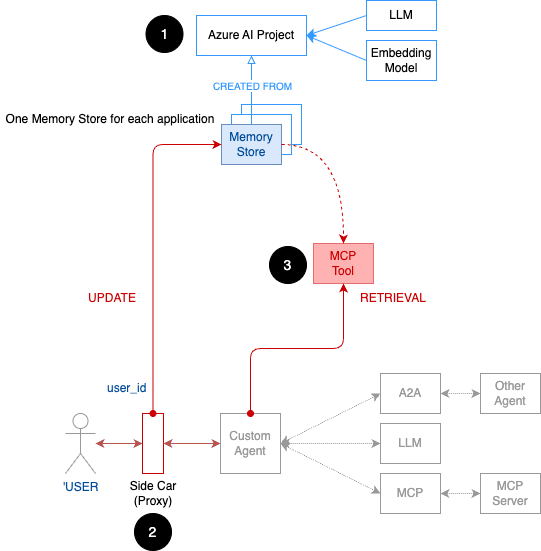
\includegraphics[width=0.8\textwidth]{docs/images/architecture.drawio.png}%
\caption{Architecture Diagram for Cortex Memory Platform}%
\label{fig:architecture}%
\end{figure}%
\vspace{\baselineskip}%
Figure \ref{fig:architecture} illustrates the architecture of the Cortex Memory Platform, which is modular, scalable, and secure. It consists of several key components that work together to provide a seamless memory management experience for users. Each component is responsible for specific tasks, and their interactions ensure that memories are created, stored, retrieved, and managed effectively. The blue boxes represent the components that are part of the Azure AI Foundry Memory Store, while the red boxes represent the additional components that we have implemented to extend its capabilities and meet the requirements of the Cortex team.
%
\par\vspace{\baselineskip}%
\begin{enumerate}[topsep=0pt]%
\item Each Kubernetes namespace has an Azure AI Foundry Service, a Large Language Model (LLM) deployment, and an embedding model deployment. The LLM and embedding model deployments are required by the Azure AI Foundry Memory Store to function, and their endpoints and secrets are configured in the Kubernetes namespace. The choice of LLM matters here. Extensive testing and evaluation are needed to determine the best model for processing and updating memory. We typically recommend OpenAI's reasoning models.%
\item In order to capture all conversations between the user and the agent, we propose a Kubernetes sidecar pod that acts as a proxy to the agent. The sidecar pod captures every conversation and forwards it to the memory store for processing and storage, ensuring that all conversations are persisted in a timely manner. This is the least intrusive way to capture conversations between the user and the agent, as it requires no changes to the agent itself. The sidecar pod can be configured to capture all conversations or only specific ones, based on the requirements of the Cortex team. Once the chat messages are captured and sent to the memory store, we delegate the processing and storage of memories to the memory store itself. The memory store uses the LLM and embedding model to analyze the conversations, extract relevant information, and store it in a structured format for easy retrieval. This frees us from having to implement our own memory store, which is a complex and time-consuming task. By leveraging the capabilities of Azure AI Foundry Memory Store, we can focus on building a robust and scalable memory platform that meets the requirements of the Cortex team.%
\item Once the memories are managed by the Azure AI Foundry Memory Store, we can implement a retrieval mechanism that lets the agent access relevant memories when needed. This is provided by the \texttt{MemorySearchPreviewTool}, which searches the memory store for relevant memories based on the current conversation context. We shall discuss the retrieval mechanism in more detail in the next section.%
\end{enumerate}%
\vspace{\baselineskip}%
\section{Retrieval Model}%
The retrieval model is a critical component of the Cortex Memory Platform, responsible for efficiently searching and retrieving relevant memories from the Azure AI Foundry Memory Store. It leverages advanced search algorithms and indexing techniques to ensure that the most pertinent memories are returned in response to user queries. The retrieval model is designed to handle large volumes of data while maintaining low latency and high accuracy, making it suitable for real-time applications where quick access to relevant information is essential. By optimizing the retrieval process, the model enhances the overall user experience and supports the effective management of memories within the platform.
%
\par\vspace{\baselineskip}%
Testing and evaluating the retrieval API is significantly complex, as it requires a large volume of test data and a variety of scenarios to ensure that the retrieval model performs well under different conditions. Whether using RAG (Retrieval-Augmented Generation) or Large Language Models (LLMs) to identify relevant memories, the retrieval model must be thoroughly tested to ensure that it meets the performance and accuracy requirements of the Cortex Memory Platform.
%
\par\vspace{\baselineskip}%
From designing the storage of memories to their retrieval mechanisms, we delegate the heavy lifting to Azure AI Foundry Memory Store, which is designed to handle these tasks. This lets us focus on building a retrieval model that efficiently searches and retrieves relevant memories from the memory store, while ensuring that the retrieval process is secure, reliable, and scalable. By leveraging the capabilities of Azure AI Foundry Memory Store, we can build a robust and effective retrieval model that meets the needs of the Cortex team and provides a seamless user experience.
%
\par\vspace{\baselineskip}%
\begin{figure}[htbp]%
\centering
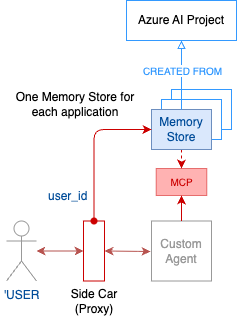
\includegraphics[width=0.4\textwidth]{docs/images/memory_store.drawio.png}%
\caption{Memory Store for an Agent}%
\label{fig:agent_memory_store}%
\end{figure}%
\vspace{\baselineskip}%
We are proposing one memory store per application (aka "agent") to simplify the retrieval model. This design choice allows us to efficiently manage and retrieve memories for each application without introducing unnecessary complexity. By having a dedicated memory store for each application, we can ensure that the retrieval model is optimized for the specific needs of that application, while also providing a clear separation of concerns between different applications.
%
\par\vspace{\baselineskip}%
\begin{figure}[htbp]%
\centering
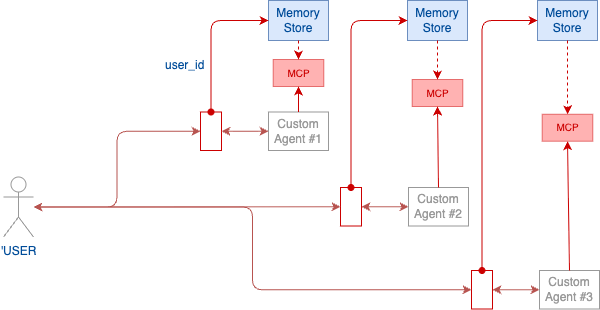
\includegraphics[width=0.8\textwidth]{docs/images/memory_stores.drawio.png}%
\caption{Memory Stores}%
\label{fig:agent_memory_stores}%
\end{figure}%
\vspace{\baselineskip}%
Figure \ref{fig:agent_memory_stores} illustrates the proposed design of having one memory store per application. Each application has its own dedicated memory store, which is responsible for storing and retrieving memories specific to that application. However, there is a caveat to this design choice. The agent can only retrieve memories from its own memory store, and cannot access memories from other applications' memory stores.
%
\par\vspace{\baselineskip}%
\begin{figure}[htbp]%
\centering
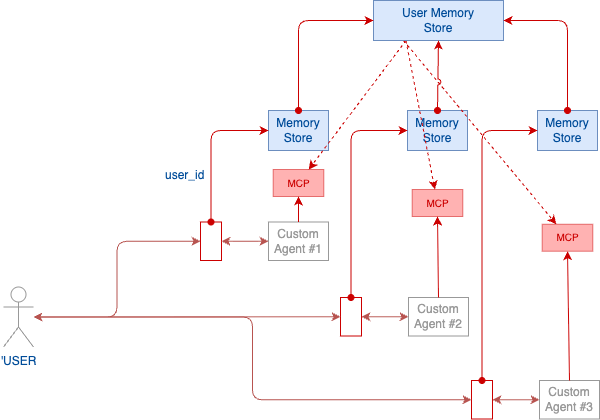
\includegraphics[width=0.8\textwidth]{docs/images/consolidate_memory_stores.drawio.png}%
\caption{Consolidated Memory Stores}%
\label{fig:consolidate_memory_stores}%
\end{figure}%
\vspace{\baselineskip}%
Figure \ref{fig:consolidate_memory_stores} shows a consolidated memory store design where all application memories are further consolidated into a common memory store, which the MCP tools for all agents can access. This design choice allows for a more centralized approach to memory management, where all memories are stored in a single location.
%
\par\vspace{\baselineskip}%
A by-product of this design choice is that the MCP tool (for retrieving memories) can offer the agent the following options:
%
\par\vspace{\baselineskip}%
\begin{enumerate}[topsep=0pt]%
\item Retrieve memories from the agent's own memory store.%
\item Retrieve memories from the consolidated memory store.%
\end{enumerate}%
\vspace{\baselineskip}%
This design choice provides flexibility in memory retrieval, letting the agent access memories from its own memory store or from the consolidated memory store, depending on the requirements of the application. These options ensure that the retrieval model is optimized for the needs of each application while still supporting a centralized approach to memory management.
%
\par\vspace{\baselineskip}%
\end{document}